% This is samplepaper.tex, a sample chapter demonstrating the
% LLNCS macro package for Springer Computer Science proceedings;
% Version 2.21 of 2022/01/12
%
\documentclass[runningheads]{llncs}
%
\usepackage[T1]{fontenc}
% T1 fonts will be used to generate the final print and online PDFs,
% so please use T1 fonts in your manuscript whenever possible.
% Other font encondings may result in incorrect characters.
%
\usepackage{graphicx}
% Used for displaying a sample figure. If possible, figure files should
% be included in EPS format.
%
% If you use the hyperref package, please uncomment the following two lines
% to display URLs in blue roman font according to Springer's eBook style:
%\usepackage{color}
%\renewcommand\UrlFont{\color{blue}\rmfamily}
%\urlstyle{rm}
\usepackage{xcolor}
\usepackage{amsmath}
\usepackage{marvosym}
\usepackage{hyperref}

\def\letter{$^{\textrm{(\Letter)}}$}

\begin{document}
%
\title{Parallel algorithm for solving multicriterial optimization problems using elements of machine learning}
%
\titlerunning{Parallel algorithm for solving multicriterial optimization problems}
% If the paper title is too long for the running head, you can set
% an abbreviated paper title here
%
\author{{Sergey Konnov\orcidID{0009-0003-4590-0870} \and
Evgeny Kozinov \Letter\orcidID{0000-0001-6776-0096} \and
Konstantin Barkalov \orcidID{0000-0001-5273-2471} \and
Alexander Sysoyev \orcidID{0000-0003-1542-7624} \and
Vladimir Grishagin\orcidID{0000-0002-2884-3670}}
}
%
\authorrunning{S. Konnov et al.}
% First names are abbreviated in the running head.
% If there are more than two authors, 'et al.' is used.
%
\institute{Lobachevsky State University of Nizhni Novgorod, Nizhni Novgorod, Russia 
\email{\{konstantin.barkalov,evgeny.kozinov\}@itmm.unn.ru}, \email{vagris@unn.ru}}
%
\maketitle              % typeset the header of the contribution
%
\begin{abstract}
Solving problems of multi-criteria optimization involves finding many combinations of optimization parameters, in which the values of the criteria cannot be improved in several criteria at once without worsening the values   of the remaining ones (Pareto set). In the framework of the research, several assumptions were introduced: criteria are multiextremal and difficult to calculate, presented in the form of a ``black box'', and the number of optimized parameters is small. The paper presents a method for solving this class of problems based on the information-statistical approach and a machine learning procedure used to increase search efficiency. A parallel implementation of the method is described, which is supplemented with the ability to perform calculations in asynchronous parallel mode. The efficiency and scalability of the proposed algorithm is analyzed on the base of solving a test class of multiextremal problems.



\keywords{Multicriterial Problems \and Global Optimization \and Machine Learning \and High Performance Computing.}
\end{abstract}
%
%
%

\section{Introduction}
\label{sec1}

%\cite{Miettinen1999,Ehrgott2005,Pardalos2017,Konnov2025,Evtushenko2014,DPA02,Durillo2010,Mostaghim2007,Nebro2009,RC05,Zitzler2001,Gergel2019_2,Gergel2018,GergelKozinov2020,Marler2004,Strongin2000,Sergeyev2013,MCO_ML_2023,scikit-learn,PyTorch,ioptmco,HV,pymoo,AGP_ML}


The problems of choosing globally optimal solutions arise when conducting a wide class of researches. To find the best options, an efficiency criterion is determined, the values   of which depend on the parameters from the permissible domain. The criterion itself can often be presented not in an analytical form, but only as a procedure for calculating its values, i.e. in the form of a ``black box'' and additionally it can be multiextremal \cite{Miettinen1999,Ehrgott2005,Pardalos2017,Strongin2000,Sergeyev2013}. For a more accurate description of the problem being solved, several (generally speaking, contradictory) optimized criteria can be taken. 

Multiextremal problems of global optimization are computationally complicated because the globally optimal solution, because in the general case, to claim that the solution is globally optimal, you need to compare it with the values of the objective function at all other points in the search area. When solving such problems using the scanning methods based on random or uniform grids, the number of calculations increases exponentially with the growth of dimensionality. It is possible to solve the considered problems using more efficient algorithms that can be divided into two large classes: deterministic \cite{Miettinen1999,Ehrgott2005,Pardalos2017,Konnov2025,Evtushenko2014} and non-deterministic (meta-heuristic) methods \cite{DPA02,Durillo2010,Mostaghim2007,Nebro2009,RC05,Zitzler2001}. 

Non-deterministic algorithms often attempt to mimic the behavior of living organisms or processes occurring in nature \cite{DPA02,Durillo2010,Mostaghim2007,Nebro2009,RC05,Zitzler2001}. Algorithms from this class do not guarantee finding the best solution with a given accuracy, but can show good efficiency when solving problems with not too many number of local extrema.

Deterministic algorithms guarantee an estimate of the globally optimal solution with a given accuracy, but in their basic implementations they can perform redundant calculations. To reduce the number of trials in this class of algorithms, heuristics are often used that reduce the amount of computations \cite{Konnov2025,AGP_ML}. Among effective deterministic algorithms for solving global optimization problems, the information-statistical family of global search methods \cite{Strongin2000,Sergeyev2013} can be considered. Initially, these algorithms were proposed for solving scalar optimization problems, subsequently, the algorithms were successfully developed to solve multicriterial problems of global search \cite{Konnov2025,MCO_ML_2023}.


In the publication \cite{Konnov2025}, we proposed an approach to solving multicriterial optimization problems that combines a classic global search algorithm with machine learning methods. In the framework of the approach, the problem of multicriterial optimization was reduced to solving a series of scalar optimization problems. In the process of solving scalar problems , a model based on machine learning methods was built and gradually improved that separated the points of effective and ineffective solutions in the criteria space. The constructed model made it possible to reduce the amount of calculations necessary to solve the problem with a given quality. Within the framework of this research, we propose the development of the approach for case when the algorithm is used on multi-core computing systems with shared memory.

The article has the following structure. Section \ref{sec2} provides a mathematical statement of the problem to be solved. Section \ref{sec3} contains a brief description of the developed algorithm and its parallel modification. Section \ref{sec4} includes the results of computational experiments demonstrating the effectiveness of the proposed approach.

\section{Problem statement}
\label{sec2}

The multicriterial optimization (MCO) problem is formulated as follows.
\begin{equation}
\label{eq:01}
  \Phi(y) = (f_1 (y),f_2 (y), \dots, f_s(y))
\end{equation}
where $f_i(y)$, $1 \leq i \leq s$, are the criteria of efficiency, $y=(y_1,y_2,\dots,y_N)$ is the vector of varied parameters, N is the dimensionality of the problem solved, and $s$ is the number of varied  criteria. It is supposed in this statement that the criteria $f_i(y)$, $1 \leq i \leq s$ are multiextremal functions, given as a ``black box'' and satisfying the Lipschitz condition
\begin{equation}
\label{eq:02}
|f_i (y') - f_i (y'')| \leq L_i \|y' - y''\| ,y',y'' \in D, 1 \leq i \leq s,
\end{equation}
where Lipschitz constants $L_i$, $1 \leq i \leq s$, are unknown \textit{a priory}.

Moreover, it is supposed that values of partial criteria $f_i(y)$, $1 \leq i \leq s$, are non-negative and their decreasing corresponds to increasing the solution efficiency. If an initial criterion does not satisfy these requirements, it is easily to build a new criterion by means of changing the sign and adding a constant for satisfying the initial requirements. Note that the constant can be selected during optimization process \cite{Konnov2025}.

It is supposed that the set of possible values of the optimized parameters $y$ is contained in the $N$-dimensional hypercube $D$:
\begin{equation}
\label{eq:03}
    D=\{y \in R^N : a_i \leq y_i \leq b_i, 1 \leq i \leq N\}
\end{equation}

As a particular solution to the MCO problem, any effective option can be considered in which it is impossible to reduce the values of all criteria at once $f_i(y)$, $1 \leq i \leq s$, by selection of parameter values $y \in D$. In general case, when solving the MCO problem, it may be necessary to find the entire set of Pareto-optimal options \cite{Miettinen1999,Ehrgott2005,Pardalos2017}.


\section{Computational scheme of the developed algorithm}
\label{sec3}

In the framework of the research, an algorithm for solving problems of multicriterial optimization with application of machine learning models has been developed. The general scheme of the algorithm is presented in Fig. \ref{fig1}. The algorithm combines elements of a deterministic global search algorithm and machine learning techniques to improve search efficiency. The following components can be pointed out in the algorithm.
\begin{enumerate}
	\item Block for accumulating and reusing the information about current state of the search.
	\item Block for building the Pareto set estimation. 
	\item Block of the global search algorithm. 
	\item Block of machine learning for building a Pareto set estimation model. 
	\item Block for the choice of trial points and implementation of computational experiments.
\end{enumerate}

Numerical solution of optimization problem consists in sequential carrying out trials (computations of criteria values at points of the search domain). The first block of the algorithm allows accumulating information about the trials performed and using it to solve problem (\ref{eq:01})-(\ref{eq:03}). Block 2 on the base of the accumulated information constructs an approximate solution as an estimate of the Pareto set. Block 3 allows efficient selection of trial points based on a global search algorithm. Block 4 builds a model for estimating the Pareto set. The built model is used to reduce the number of trials required to find the Pareto set with high quality and with fewer trials. The fifth block contains an algorithm that allows realizing trials in parallel. Let's take a closer look at the computing blocks.

\begin{figure}[t]
\center
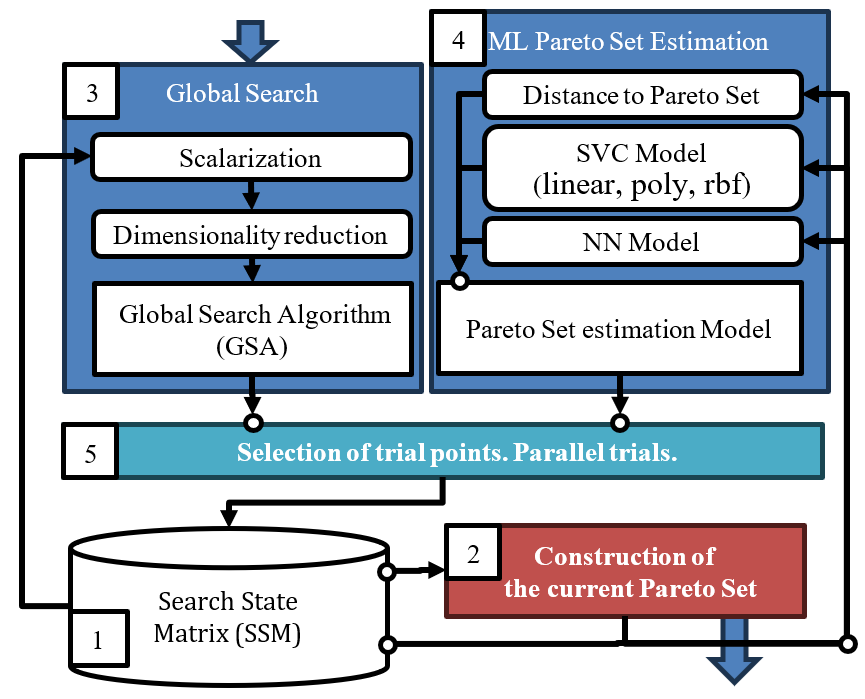
\includegraphics[width=0.6\textwidth]{fig1.png}
\caption{Computational scheme of the algorithm for solving multicriterial optimization problems using machine learning models.} \label{fig1}
\end{figure}


\subsection{Block of the global search algorithm}
\label{subsec31}

The search for a globally optimal solution to problem (\ref{eq:01})-(\ref{eq:03}) consists of the following basic steps:
\begin{enumerate}
	\item scalarization of efficiency criteria;
	\item dimensionality reduction;
	\item optimization on the base of the global search algorithm.
\end{enumerate}

\textbf{Scalarization of efficiency criteria.} It is possible to find the Pareto set either solving the problem in the original formulation \cite{Evtushenko2014,DPA02,Durillo2010,Mostaghim2007,Nebro2009,RC05,Zitzler2001}, or reducing the original problem to a series of scalar problems to find effective solutions \cite{Pardalos2017,Konnov2025,Gergel2019_2,Gergel2018,GergelKozinov2020}. 

In the framework of the developed approach \cite{Konnov2025}, the second option with scalarization of criteria is used. To build a good estimate of the Pareto set, a family of problems
\begin{equation}
\label{eq:04}
\min {\varphi_j (y)}=F(\lambda_j,y),F(\lambda_j,y) \in \{F(\lambda_1,y),F(\lambda_2,y),\dots,F(\lambda_\tau,y)\},y\in D,
\end{equation}
is solved,  where $F(\lambda_j,y)$, $1 \leq j \leq \tau$, is a multiextremal function, obtained on the base of scalarization of criteria $f_i(y)$, $1 \leq i \leq s$. Here $\lambda_j=\{\lambda_{i,j}\}$, $1 \leq i \leq s$, $1 \leq j \leq \tau$, are significance indicators for each criterion, s is the number of criteria, $\tau$ is the number of scalar optimization problems. There are different ways to build functions $F(\lambda_j,y)$ \cite{Miettinen1999,Konnov2025,Marler2004}.  
%В рамках предлагаемого алгоритма $\tau$ фиксируеться. Множество наборов $\lambda_j$, $1 \leq j \leq \tau$, выбирается случайно с использованием генератора Соболя в множестве  возможных значений (\ref{eq:051}). 
{\color{red} In the proposed algorithm, $\tau$ is fixed. The set of $\lambda_j$, $1 \leq j \leq \tau$, is chosen randomly using the Sobol generator\cite{Sobol2003} in the space of possible values (\ref{eq:051})}

\begin{equation}
\label{eq:051}
\sum_{i=1}^s {\lambda_{i,j}} = 1, 0 \leq \lambda_{i,j} \leq 1.
\end{equation}

The performed computational experiments used minimax convolution of criteria

\begin{equation}
\label{eq:05}
F(\lambda_j, y) = \max_{1 \leq i \leq s} \left(\lambda_{i,j} f_i (y)\right), y \in D.
\end{equation}

\textbf{Dimensionality reduction.} For solving optimization problems (\ref{eq:04}) the dimensionality reduction on the base of Peano curves $y(x)$ that map unambiguously and continuously the segment $[0,1]$ to the $N$-dimensional hypercube $D$ is used \cite{Konnov2025,Gergel2019_2,GergelKozinov2020}. As a result of this reduction, multidimensional global optimization problems (\ref{eq:04}) are reduced to one-dimensional subproblems
\begin{equation}
\label{eq:06}
\min_x {\varphi_j(y(x))} = \min_y {\varphi_j(y)}, x \in [0,1], y \in D, 1 \leq j \leq \tau
\end{equation}

Note that the reduced one-dimensional functions $\varphi_j (y(x))$ from (\ref{eq:06}) satisfy the H{\" o}lder condition, i.e.
\begin{equation}
\label{eq:07}
|\varphi_j(y(x')) - \varphi_j(y(x''))| \leq H |x' - x''|^{1/N} , x \in [0,1],
\end{equation}
where the constant $H$ is given as $H=2L\sqrt{N+3}$, and $L$ is the Lipschitz constant from (\ref{eq:02}).

\textbf{Global search algorithm.} Information-statistical algorithm of global search (shortly GSA) \cite{Konnov2025,Gergel2019_2,Gergel2018,GergelKozinov2020,Strongin2000,Sergeyev2013} is used to solve problems (\ref{eq:06}). The computational scheme of GSA is as follows. At each iteration of the global search, one trial (calculation of the value of the optimized function $\varphi_j (x)$ from (\ref{eq:06})) is executed. In the first iteration, two tests are carried out at the ends of the interval $x^0=0$,$x^1=1$. Let $k$, $k>2$, iterations of the global search be performed. The selection of the next test point is based on the following rules.

\textit{Rule 1.} Renumber search iteration points with subscripts in order of increasing coordinate values
\begin{equation}
    \label{eq:08}
    0 = x_0 < x_1 < \dots < x_i < \dots < x_{k} = 1
\end{equation}
\textit{Rule 2.} Calculate the current estimate of the H{\" o}lder constant from (\ref{eq:07}) for the reduced function $\varphi_j (x)$:
\begin{equation}
    \label{eq:9}
		\begin{matrix}
		m=\begin{cases}
				\begin{matrix}
					 r M, & M >0 \\
					 1, & M = 0 
				\end{matrix} \; , 
			\end{cases}
		M = \max_{1 \leq i \leq k} \frac{| z_i - z_{i-1}|}{\varrho_i}, \\
		z_i = \varphi_j( y(x_i) ), \varrho_i=\sqrt[N]{x_i-x_{i-1}}
		\end{matrix}
\end{equation}
where $r$, $r>1$, is the reliability parameter of the algorithm. 

\textit{Rule 3.} Compute characteristics $R(i)$ for each interval $(x_{i-1}, x_i)$, $1\leq i \leq k$, according to the expression
\begin{equation}
    \label{eq:10}
    R(i) = \varrho_i + \frac{(z_i-z_{i-1})^2}{m^2 \varrho_i} - \frac{2 (z_i+z_{i-1})}{m}, 1 \leq i \leq k.
\end{equation}

\textit{Rule 4.} Select the interval with the maximal characteristic $R(i)$ from (\ref{eq:10})
\begin{equation}
    \label{eq:11}
    R(t) = arg\max_{1 \leq i \leq k} {R(i)}.
\end{equation}

\textit{Rule 5.} Execute the next trial in the interval with the maximal characteristic value, according to the expression
\begin{equation}
    \label{eq:12}
    x^{k+1} = \frac{x_t + x_{t-1}}{2} - sign(z_t - z_{t-1}) \frac{1}{2r} \left[\frac{|z_t - z_{t-1}|}{m} \right]^N
\end{equation}

The stopping condition of the algorithm, according to which the execution of the algorithm for the current global search problem (\ref{eq:06}) is terminated, consists in achieving the required accuracy of solving the problem, i.e.
\begin{equation}
    \label{eq:13}
    \varrho_t < \varepsilon.
\end{equation}



\subsection{Block for accumulating and reusing the information about current state of the search}
\label{subsec32}

As mentioned earlier, the numerical solution to optimization problems consists in sequential realization of trials $z^i=\varphi_j (y^i)$ from (\ref{eq:04}) at points $y^i$, $1 \leq i \leq k$, of the search domain $D$. The obtained data can be presented in the form of \textit{the search information set} (SIS):
\begin{equation}
    \label{eq:14}
    \Omega_k=\{\mu^i=(y^i,f^i=f(y^i))^T: 0 \leq i \leq k\}
\end{equation}

SIS contains all available information about the solved problem MCO (\ref{eq:01})-(\ref{eq:03}). Improved search efficiency can be achieved on the base of information available in $\Omega_k$. In our approach SIS is used:
\begin{enumerate}
	\item	when the scalar statement of the problem (\ref{eq:04}) is changed,
	\item	during building a Pareto set estimate, 
	\item	in the process of building a machine learning model based on the Pareto set.
\end{enumerate}

Within item 1 the following sequence of actions is performed. When task (\ref{eq:06}) is changed, new coefficients $\lambda_{j+1}$ from (\ref{eq:04}) are selected. Further, scalarization of the vector criterion (\ref{eq:04}) and dimensionality reduction (\ref{eq:06}) transform SIS from (\ref{eq:14}) to the form used in the optimization process (\ref{eq:08})-(\ref{eq:13}) for the current problem (\ref{eq:04}). Transformation uses already calculated criteria values and new coefficients $\lambda_{j+1}$. As a consequence, the recount does not take long time. Thus, information about the calculated criteria is not lost when changing the task statement, but is reused. This approach has shown its effectiveness in solving many problems \cite{Konnov2025,Gergel2018,GergelKozinov2020}.

The calculations fulfilled under items 2 and 3 are described in sections \ref{subsec33} and \ref{subsec34} respectively.

\subsection{Block for building the Pareto set estimation}
\label{subsec33}

Accumulation of search information allows more accurate estimation of the Pareto set. In solving the series of problems (\ref{eq:04}), after each trial performed or task setting change, the current Pareto set is selected on the base of all the trials executed. Thus, even when solving one optimization problem from (\ref{eq:04}), the Pareto set evaluation contains several variants of solutions, from which the researcher can choose the best variant for himself (see Fig. \ref{fig2}, blue dots). Solving additional tasks (\ref{eq:04}) makes it possible to improve the found solution (see Fig. \ref{fig2}).

\begin{figure}[t]
\center
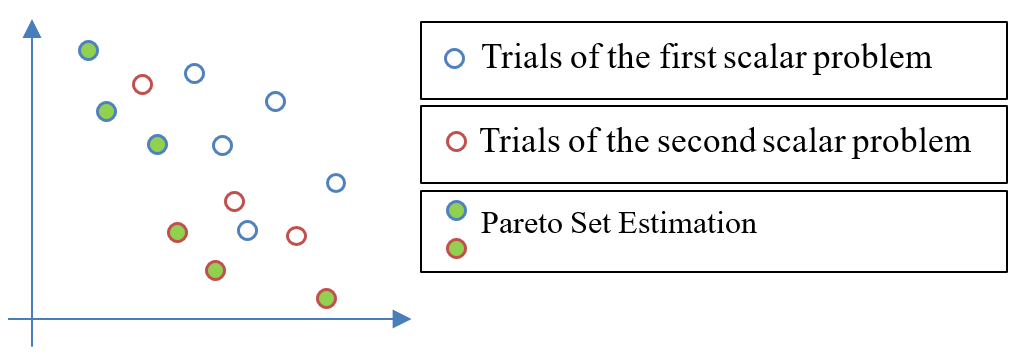
\includegraphics[width=0.7\textwidth]{fig2.png}
\caption{Example of Pareto set evaluation in solving two scalar optimization problems (trial points are presented in the criteria space).} \label{fig2}
\end{figure}


\subsection{Block of  building the machine learning for estimation of the Pareto set}
\label{subsec34}

To improve the search efficiency within the developed scheme, the calculation of characteristics for intervals (\ref{eq:10}) is changed to the following dependence \cite{Konnov2025}:
\begin{equation}
    \label{eq:15}
    R(i) = R_{GSA} (i) +  \alpha R_{PS} (i)
\end{equation}

The characteristic $R_{GSA}(i)$ from (\ref{eq:15}) is used to find the global minimum in the current optimization problem. The method of calculating $R_{GSA}(i)$ corresponds to rule 3 of the GSA in formula (\ref{eq:10}). The value of $R_{PS}(i)$ is calculated on the base of the found Pareto set in the current optimization step and links solvable optimization problems from the set (\ref{eq:04}). The coefficient $\alpha$ changes the degree of influence of the characteristic  $R_{PS}(i)$ on the choice of the next point. At low $\alpha$ values, the algorithm executes more trials to find the optimal solution of the current optimization problem (\ref{eq:04}). At high $\alpha$ values, a new trial is carried out in the vicinity of the Pareto set. 

To calculate the value of $R_{PS}(i)$, we propose using machine learning methods. Various algorithms for calculation of  $R_{PS}(i)$ have been proposed in \cite{Konnov2025}. All proposed methods use the following scheme. In the course of solving the MCO problem, after every changing the coefficients  $\lambda_j$, $1 \leq j \leq \tau$, and therefore, moving to a new optimization problem from (\ref{eq:06}), all obtained trial points (\ref{eq:14}) are divided into two classes. The first class includes points belonging to the Pareto set. All other trial points belong to the second class. The quantity of points that do not belong to the Pareto set, as a rule, is significantly larger; therefore, the classes are not balanced. For more efficient work of machine learning algorithms, weights corresponding to the significance of trial points are set for each class, if possible. After training the model in the selected classes, the following approaches are used for building $R_{PS}(i)$.
\begin{enumerate}
	\item When using the Support Vector Classification (SVC) model with a linear kernel, $R_{PS}(i)$ is considered on the base of the distance to the dividing hyperplane.
	\item	When using the SVC model with an arbitrary kernel, $R_{PS}(i)$ RP is built according to probabilities of belonging trial points to the first class (Pareto set).
	\item Neural network models are used as a new way to evaluate $R_{PS}(i)$. The method of calculating $R_{PS}(i)$ is similar to step 2.
\end{enumerate}

In the framework of the first approach, an SVC model with a linear kernel is built for computation $R_{PS}(i)$. Information is extracted from the model to construct a dividing hyperplane equation between the selected point classes in the criteria value space. The characteristic $R_{PS}(i)$ of the interval $[x_{i-1},x_i ]$ is considered as the sum of the distances of the criteria values  from the points $x_{i-1}$, $x_i$ to the hyperplane. The value below the hyperplane is taken with a plus sign, and above the hyperplane  with a minus sign.

In the second approach, the probability of belonging  each of the points to the Pareto region is used instead of distances. $R_{PS}(i)$ is considered as the arithmetic mean of the calculated probability values for the points $x_{i-1}$ and $x_i$. This approach is more universal, since the counting method does not depend on the selected kernel. The method of calculating $R_{PS}(i)$ is described more detailed in \cite{Konnov2025}.

The third approach is based on the second one and uses new models based on fully connected neural networks. Two variants of models were considered.
\begin{enumerate}
	\item Variant with two hidden layers (Fig. \ref{fig3}, a). In this case, the Input layer consists of $N$ nodes, where the number $N$ must be equal to the number of criteria in the problem being solved. The first hidden layer contains 128 nodes, the second hidden layer includes 64 nodes, output layer consists of 2 nodes, each of which denotes the probability of assigning a point to one of the classes describing belonging to the Pareto set. The ReLU function was used as the activation function after the Input layer and the first hidden layer. To obtain the probability before the output layer, the softmax function is applied to the data.
	\item Variant with one hidden layer (Fig. \ref{fig3}, b).  This is a simpler option, in which the Input layer also consists of N nodes, where N is equal to the number of criteria. The next (hidden) layer contains 100 nodes. The last (output) layer also consists of 2 layers. Similar to the previous case, the activation function is ReLU, and before the output layer, the softmax function is applied.
\end{enumerate}

\begin{figure}[t]
\center
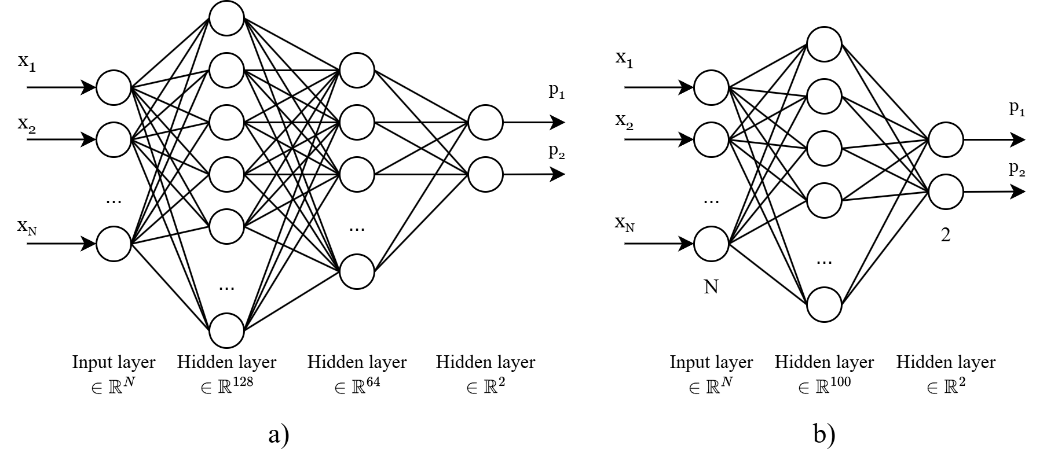
\includegraphics[width=0.8\textwidth]{fig3.png}
\caption{Neural network models used to calculate the characteristic $R_{PS}(i)$.} \label{fig3}
\end{figure}

Fig. \ref{fig4} shows an example of built functions $R_{PS}(i)$ in the criteria domain. Red denotes the points assigned by the algorithm to the Pareto set. Graph (a) refers to the first approach with the calculation of distances to the hyperplane. Plots (b), (c), (d) demonstrate results for the second approach using SVC models to calculate probabilities. Graphs (e), (f) show heat maps for the third approach using neural network models.

From the figure, it can be seen that the function $R_{PS}(i)$ for each of the considered variants differs in the quality of the evaluation of Pareto sets. When choosing a machine learning model, it should be taken into account that building a model with a good description of the domain may require more computing resources. An analysis of the impact of the selected model on the quality of the resulting solution is presented in Section \ref{sec4} with the results of computational experiments. Note that numerous computational experiments have shown that changing the method of calculating characteristic (\ref{eq:15}) leads to a significant increase in the efficiency of the algorithm as a whole \cite{Konnov2025,MCO_ML_2023}.

\begin{figure}[t]
\center
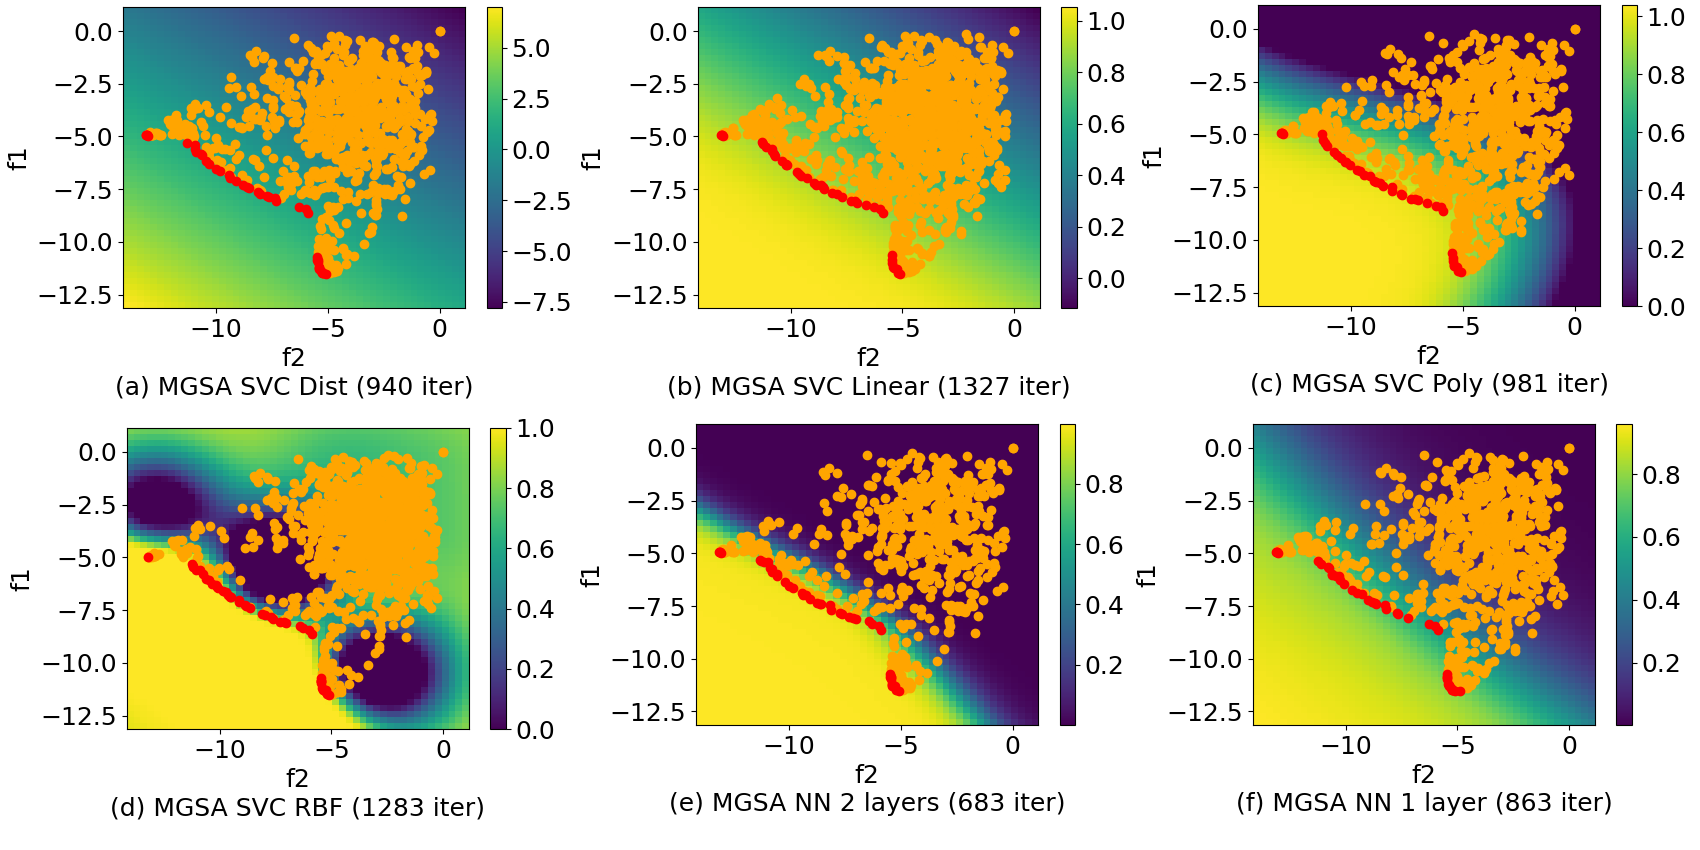
\includegraphics[width=\textwidth]{fig4.png}
\caption{Examples of Pareto set evaluation for the case of two scalar optimization problems.} \label{fig4}
\end{figure}


\subsection{Block for the choice of trial points and implementation of computational experiments}
\label{subsec35}

To further improve the search efficiency, a parallel calculation scheme has been implemented as a new element of the algorithm for solving multicriterial optimization problems using machine learning \cite{ioptmco}. 

In global search algorithms, the traditional method of parallelization by dividing the search area into parts is not effective, since the minimum values of the criteria can fall into a limited number of subregions, therefore, many trials would not improve the Pareto set estimation. 
In this work, the classic master-working circuit is used as a parallel scheme. 

Workflows are waiting for a new trial point or command to complete calculations. When a point is received, criteria calculations are performed and the master is notified of the results. 

The scheme of the master is as follows. Let there be $p$ workflows. The first $p$ trials are executed in parallel at points $x_0=0<x_1<\dots<x_i<\dots<x_{p-1}=1$, $0<i<p$, uniformly distributed on the segment $[0,1]$. Further, in the case when all workflows are busy, the master is in the waiting state. When information from the workflow appears, the master obtains the value of the criteria from (\ref{eq:06}) and updates the set of search information (\ref{eq:14}), calculates the estimate of the H{\" o}lder constant (\ref{eq:07}) as well as the values of the characteristics of the intervals (\ref{eq:15}). As in the case of a sequential implementation, it selects the interval with the maximal characteristic, and also computes the trial point (\ref{eq:12}). The obtained value is sent to the workflow to continue the computations. To avoid repeated calculations, intervals already involved in calculations on workflows are not involved in the calculation of characteristics.

As in the sequential algorithm, stopping and evaluating the resulting solution is carried out according to rule (\ref{eq:13}). A detailed analysis of the effectiveness of the given parallel implementation is presented in Section \ref{sec4} with computational experiments.


\section{Results of computational experiments}
\label{sec4}

Computational experiments were carried out on the nodes of the Lobachevsky supercomputer of Nizhny Novgorod State University with two processors Intel Xeon Silver 4310T 2.3 GHz, 64 GB RAM. Machine learning libraries SciKit-Learn 0.24.2 \cite{scikit-learn} and PyTorch 2.5.1 \cite{PyTorch} were used in experiments. The algorithm proposed in the work was implemented in Python using the framework iOpt \cite{ioptmco}. 
%Сравнение предыдущей последовательной версии предлагаемого алгоритма с современными разработками можно найти в нашей статье [Konnov2025]. В этом разделе больше внимания уделено анализу эффективности параллельной реализации.
{\color{red}  A comparison of the previous sequential version of the proposed algorithm with state-of-the-art developments can be found in our paper \cite{Konnov2025}. This section focuses more on the analysis of the efficiently of parallel implementation.}

As a criterion for the quality of the found Pareto set, the indicator HV was applied. Higher value of the indicator corresponds to better solution. 
HV index is a traditional quality metric when approximating a Pareto set \cite{Evtushenko2014,pymoo,AGP_ML}.
To assess the performance of the algorithm, the number of trials carried out when solving the problem are given. However, when solving complex optimization problems, one trial can take a significant time. In such conditions, the reduction of the number of trials reduces the total computation time in general. In the presented experimental results, the number of trials spent on solving each problem and the HV indicators were averaged according to the number of solved problems.

To estimate the quality of the resulting solutions, a number of computational experiments were performed to solve 100 unconstrained two-criteria two-dimensional MCO problems. The following multi-extremal functions \cite{Gergel2019_2}:
\begin{equation}
    \label{eq:16}
		\begin{matrix}
		  f(y)= -(AB + CD)^{1/2}, \\
			AB =(\sum_{i=1}^7{\sum_{j=1}^7{[A_{ij} a_{ij} (y_1,y_2) + B_{ij} b_{ij} (y_1,y_2)])}})^2, \\
			CD =(\sum_{i=1}^7{\sum_{j=1}^7{[C_{ij} a_{ij} (y_1,y_2) - D_{ij} b_{ij} (y_1,y_2)])}})^2, \\
			a_{ij} (y_1,y_2) = \sin(\pi i y_1) \sin(\pi j y_2), \\
			b_{ij} (y_1,y_2) = \cos(\pi i y_1) \cos(\pi j y_2),
		\end{matrix}
\end{equation}
were used as partial criteria in the two-criteria statement, where $0 \leq y_1, y_2 \leq 1$, parameters $-1 \leq A_{ij},B_{ij},C_{ij},D_{ij} \leq 1$ are independent uniformly distributed random values.

Results of the experiments for the following algorithms are presented (see subsection \ref{subsec34}):
\begin{enumerate}
	\item MGSA -- machine learning elements are not used,
	\item MGSA Dist -- the modified algorithm with computation $R_{PS}(i)$ from (\ref{eq:15}) based on distances,
	\item MGSA Linear SVC, MGSA Poly SVC, MGSA Rbf SVC -- the algorithm modification with computation $R_{PS}(i)$ from (\ref{eq:15}) based on probabilities with different SVC algorithm kernel,
	\item MGSA NN -- the algorithm modification with computation $R_{PS}(i)$ from (\ref{eq:15}) on the base of probabilities obtained using neural networks.
\end{enumerate}
	
Fig. \ref{fig5} shows the dependence of the average value of the HV index on the average number of trials for the sequential algorithm. The number of $\lambda$ values from (\ref{eq:04}) was equal to $\tau=50$ in all experiments. The $\lambda$ values were chosen to be uniformly distributed over the interval [0,1]. Several solution accuracy values $\varepsilon = \{0.1,0.05,0.01\}$ were fixed for plotting the graph for algorithm (\ref{eq:13}). 100 problems were solved for each accuracy value and the average results were plotted on a graph. The position of the resulting curve for the chosen algorithm to the left and above corresponds to the best behavior of the algorithm as a whole. During the experiments the parameter $\alpha$ from (15) varied within the range $[0.01,0.05]$ with a step of $0.01$, Fig. \ref{fig5} shows only the best results for each of the variants.



\begin{figure}[t]
\center
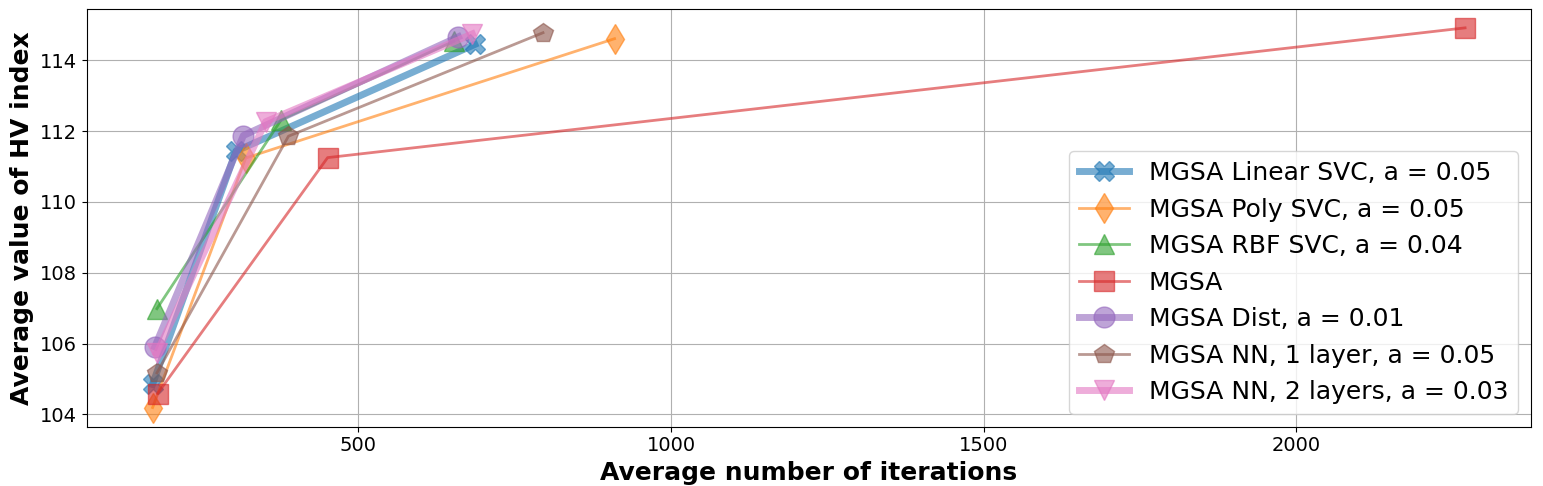
\includegraphics[width=0.8\textwidth]{fig5.png}
\caption{Comparison of HV index values for sequential algorithm implementation.} \label{fig5}
\end{figure}

Based on the results of experiments with sequential implementation, all approaches using machine learning models exceed the MGSA algorithm by more than two times. Modifications of the algorithm can be distinguished that demonstrate the best results both in terms of the average number of iterations and in terms of the average HV. These include approaches using SVC (Linear, Rbf kernels), a distance calculation approach, and neural networks with two hidden layers. Modification with one hidden layer shows slightly worse results. Modification  MGSA Poly SVC with polynomial kernel showed least improvement over MGSA. It is also worth noting that the modification of the MGSA Rbf SVC algorithm in the case of low accuracy demonstrates the best quality.

Next, consider a parallel version of the algorithm (see subsection \ref{subsec35}). Table \ref{tab:1} shows the results of the average value of the trial number per process by tasks for each of the models in dependence on the number of processes. Accuracy $\varepsilon=0.01$ was used in the experiment. The number of processes used is indicated in the first row of the table. The three best modifications of the algorithm in terms of the average number of trials per process are shown in bold.

% Please add the following required packages to your document preamble:
% \usepackage{graphicx}
\begin{table}[t]
\centering
\caption{Average number of trials per process}
\label{tab:1}
\resizebox{0.8\textwidth}{!}{%
\begin{tabular}{ccccccc}
\hline
\textbf{Number of processes}            & \textbf{1}      & \textbf{2}      & \textbf{4}      & \textbf{8}      & \textbf{16}    & \textbf{20}    \\ \hline
MGSA                                    & 2269.82         & 1385.02         & 746.57          & 373.36          & 202.01            & 143.52         \\
\textbf{MGSA   Linear SVC,  $\alpha$ = 0.05}   & \textbf{686.13} & \textbf{408.79} & \textbf{213.6}  & \textbf{111.85} & \textbf{70.95} & \textbf{62.16} \\
MGSA Poly SVC, $\alpha$ = 0.05               & 909.59          & 544.19          & 278.62          & 153.64          & 95.37          & 77.94          \\
MGSA RBF SVC, $\alpha$ = 0.04                & 652.74          & 446.84          & 233.81          & 119.84          & 72.36          & 62.37          \\
\textbf{MGSA Dist, $\alpha$ = 0.01}          & \textbf{659.98} & \textbf{402.9}  & \textbf{211.33} & \textbf{112.38} & \textbf{70.79} & \textbf{62.00} \\
MGSA NN 1 layer, $\alpha$ = 0.05             & 795.16          & 446.25          & 232.08          & 117.16          & 75.19          & 62.70          \\
\textbf{MGSA NN 2 layers, $\alpha$ =   0.03} & \textbf{682.12} & \textbf{401.74} & \textbf{219.62} & \textbf{113.32} & \textbf{73.51} & \textbf{61.32} \\ \hline
\end{tabular}%
}
\end{table}

According to Table \ref{tab:1}, MGSA Dist, MGSA Linear SVC and MGSA NN algorithms with two hidden layers demonstrate the best results. To analyze the quality of the resulting solution, the values   of the HV index are given in Table \ref{tab:2}. The table also shows three best modifications.

\begin{table}[t]
\centering
\caption{Average HV Index in dependence on number of processes}
\label{tab:2}
\resizebox{0.8\textwidth}{!}{%
\begin{tabular}{ccccccc}
\hline
Number of processes                   & \textbf{1}      & \textbf{2}      & \textbf{4}      & \textbf{8}      & \textbf{16}     & \textbf{20}     \\ \hline
\textbf{MGSA}                         & \textbf{114.91} & \textbf{114.79} & \textbf{114.84} & \textbf{114.90} & \textbf{115.00} & \textbf{114.96} \\
MGSA Linear SVC, $\alpha$ = 0.05           & 114.44          & 114.65          & 114.72          & 114.74          & 114.91          & 114.96          \\
\textbf{MGSA   Poly SVC, $\alpha$ = 0.05} & \textbf{114.61} & \textbf{114.64} & \textbf{114.71} & \textbf{114.8}  & \textbf{114.95} & \textbf{115.01} \\
MGSA RBF SVC, $\alpha$ = 0.04           & 114.54          & 114.54          & 114.73          & 114.89          & 114.92          & 114.96          \\
MGSA Dist, $\alpha$ = 0.01                 & 114.66          & 114.55          & 114.69          & 114.73          & 114.92          & 114.93          \\
MGSA NN 1 layer, $\alpha$ = 0.05           & 114.77          & 114.61          & 114.72          & 114.81          & 114.96          & 114.98          \\
\textbf{MGSA NN 2 layers, $\alpha$ = 0.03} & \textbf{114.74} & \textbf{114.54} & \textbf{114.71} & \textbf{114.76} & \textbf{114.98} & \textbf{115.01} \\ \hline
\end{tabular}%
}
\end{table}

From Table \ref{tab:2} as a whole, it can be concluded that parallel modification of the algorithm does not worsen the quality of the found solution. For a more detailed productivity analysis let's plot the graph by analogy with Fig. \ref{fig5} for the case of 20 processes.

\begin{figure}[t]
\center
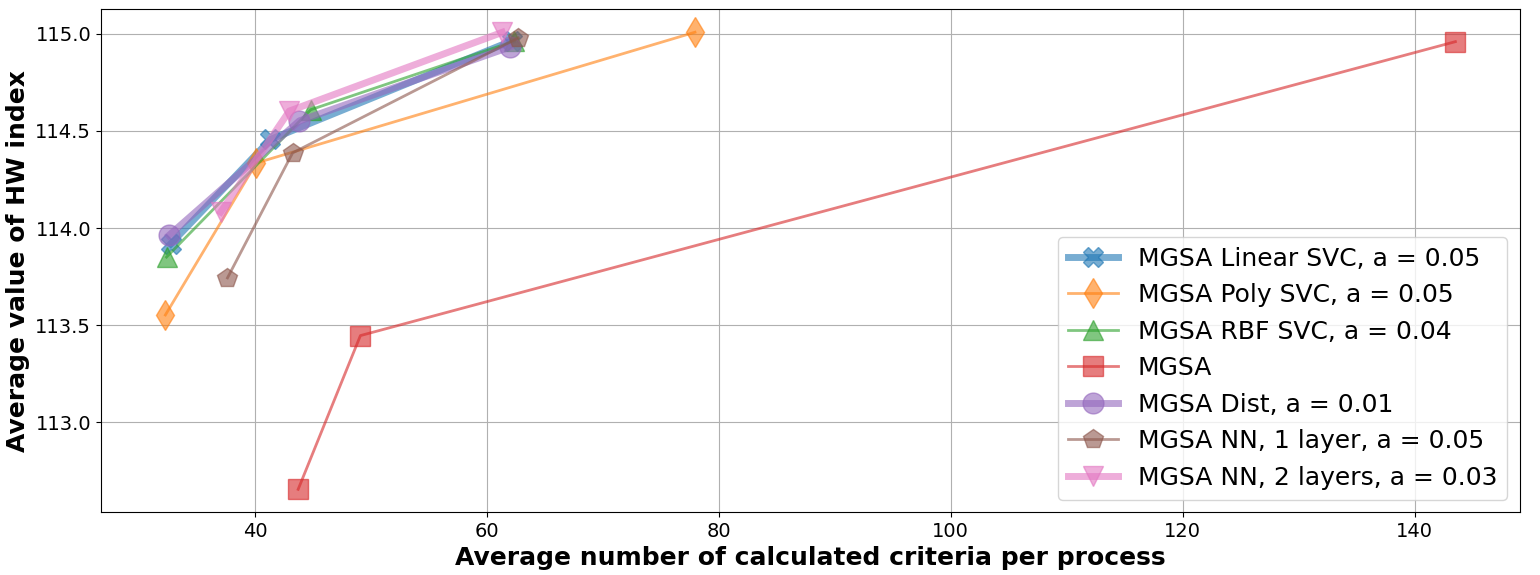
\includegraphics[width=0.8\textwidth]{fig6.png}
\caption{Dependence of the mean value of the index HV from the trial number per process for the case of 20 processes.} \label{fig6}
\end{figure}

Fig. \ref{fig6} demonstrates that as the number of processes used increases, all algorithms are significantly ahead of the MGSA method, which does not use machine learning models, in both the average number of trials per process and the HV indicator, especially if high solution accuracy is to be ensured. All modifications of the algorithm except MGSA Poly SVC and MGSA NN with one layer show similar quality. A simpler modification MGSA NN with one hidden layer with a small number of trials lags behind in quality and aligns with the rest when increasing the number of trials. This may indicate that this model can be useful when high-precision calculations are needed, in other cases it is recommended to use other machine learning models. At the same time, a simple model can learn much faster.

Fig. \ref{fig7} shows the value of the HV index depending on the number of trials when the number of used processes changes. Since MGSA NN 2 layers demonstrates better results than MGSA NN 1 layer, the information about the last modification are not given. 

According to Fig. \ref{fig7}, all presented models show a significant increase in the HV index and a decrease in the trial number per process when increasing the number of processes. Approach without using machine learning methods demonstrate similar dynamics when the target accuracy is high, however, at lower values, changes in the number of counted criteria on one process become less noticeable. It is also worth noting that, unlike the basic MGSA algorithm, all modifications with machine learning elements do not lose quality when switching to a parallel implementation.


\begin{figure}[t]
\center
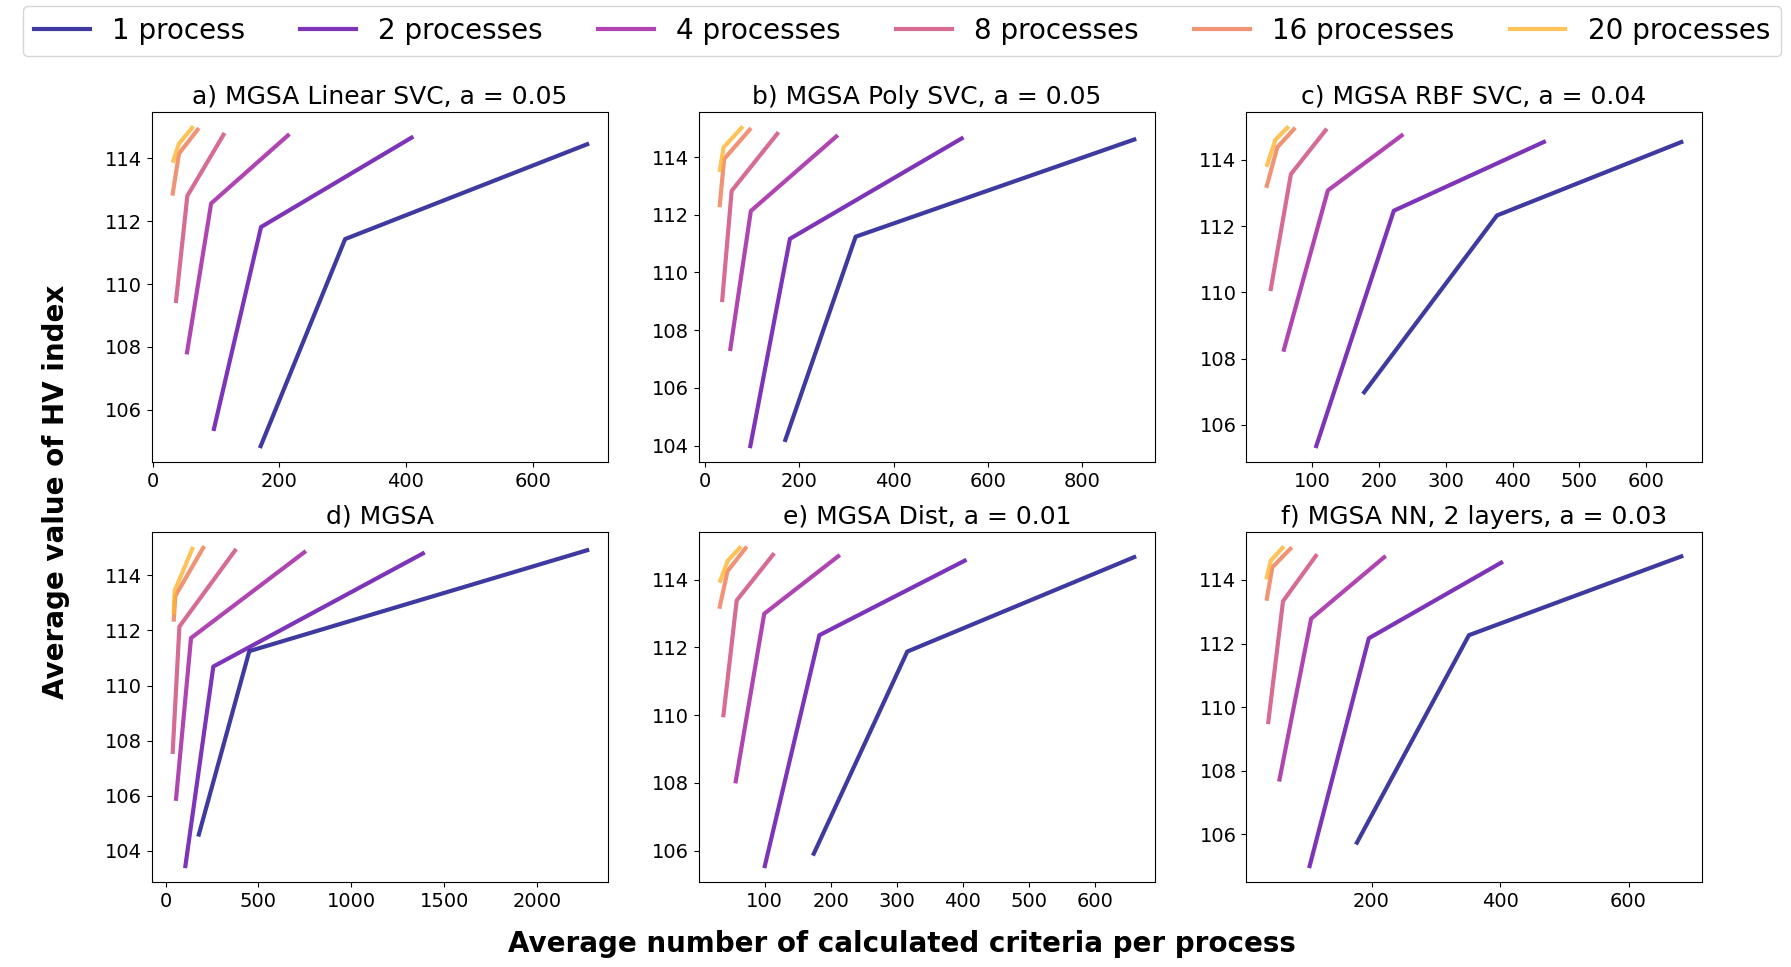
\includegraphics[width=0.8\textwidth]{fig7.png}
\caption{Dependence of the HV index on the number of trials executed for different number of processes.} \label{fig7}
\end{figure}


\section{Conclusion}
\label{sec5}
The research presents a parallel modification of the global search algorithm for solving multicriterial optimization problems. One of the features of the algo-rithm is the combination of the classic global search algorithm with machine learning methods. The combination of algorithms shows high efficiency in both sequential and parallel modifications. As the direction of further research it is planned to organize a number of experiments to solve applied problems and compare search efficiency with a number of third-party frameworks.


\begin{credits}
\subsubsection{\ackname} The study  is supported by the program for the development of regional scientific and educational mathematical centers, Agreement No 075-02-2025-1727 with additional agreement No 075-02-2025-1727/1.

\subsubsection{\discintname}
The authors have no competing interests to declare that are relevant to the content of this article.
\end{credits}
%
% ---- Bibliography ----
%
% BibTeX users should specify bibliography style 'splncs04'.
% References will then be sorted and formatted in the correct style.
%
\bibliographystyle{splncs04}
\bibliography{bibliography}
%
%\begin{thebibliography}{8}
%\bibitem{ref_article1}
%Author, F.: Article title. Journal \textbf{2}(5), 99--110 (2016)
%
%\bibitem{ref_lncs1}
%Author, F., Author, S.: Title of a proceedings paper. In: Editor,
%F., Editor, S. (eds.) CONFERENCE 2016, LNCS, vol. 9999, pp. 1--13.
%Springer, Heidelberg (2016). \doi{10.10007/1234567890}
%
%\bibitem{ref_book1}
%Author, F., Author, S., Author, T.: Book title. 2nd edn. Publisher,
%Location (1999)
%
%\bibitem{ref_proc1}
%Author, A.-B.: Contribution title. In: 9th International Proceedings
%on Proceedings, pp. 1--2. Publisher, Location (2010)
%
%\bibitem{ref_url1}
%LNCS Homepage, \url{http://www.springer.com/lncs}, last accessed 2023/10/25
%\end{thebibliography}
\end{document}
